\documentclass[../main.tex]{subfiles}

\begin{document}

\subfile{introduction}

\part{Model Predictive Control: Decomposition and Security}

\chapter[Decomposing the Model Predictive Control]{Decomposing the\\ Model Predictive Control}
\epigraph{\centering The mystery of the universe \\ is not time but size.}
{\textit{The Gunslinger}\\\textsc{Stephen King}}

\minitoc

\section{Model Predictive Control}
Model Predictive Control, or even \mpc, is a closed-loop control strategy based
on the solution of optimization problems.
Given a system model and an objective function, this strategy uses the system model to predict future states and compute a control sequence that optimizes the given objective function.
Since the solution is found by using optimization problems, it is natural to add some restrictions on the system, which are usually defined as (in)equality constraints.

The fact that constraints can be easily added to the specifications gave it a special place in the industry, where is largely used in a plethora of applications (\todo{add uses of MPC in the industry}).

As it is generally implemented through a digital computer, we assume the system we want to control to be modeled in discrete time with dynamics
\begin{equation}
\vec{x}[k+1]=f(\vec{x}[k],\vec{u}[k]),
\end{equation}
where $\vec{x}[k]:\R^{n_{x}}$ is the state of the system and $\vec{u}[k]:\R^{n_{u}}$ is the input of the system.

The system can be under constraints
\begin{equation}
 h(\vec{x}[k],\vec{u}[k])\preceq\0,
\end{equation}
with $h:\R^{n_{x}}\times\R^{n_{u}}\to\R^{n_{c}}$. Observe that mathematically equality constraints can be represented by a couple of inequality constraints, although for implementation in computers it can lead to poor numerical conditioning, resulting unexpected behavior~\cite{BorrelliEtAl2017}.

Given an objective function $J:\R^{n_{x}}\times\R^{N\cdot n_{u}}\to \R$, we can optimize this objective for a given horizon $\set{H}=\{1\mathbin{:}N\}$ to obtain a control sequence $\vec{U}[k]=[\vec{u}[k|k]\T \dots \vec{u}[k+N-1|k]\T]$, where
we use states and input predictions of time $k+i$ calculated in a time $k$, represented by $\vec{x}[k+i|k]$ and $\vec{u}[k+i|k]$. The problem solved to calculate the control sequence is

\begin{equation}\label{eq:general_mpc}
  \small
  \begin{aligned}
    \begin{matrix}
      \underset{\vec{U}[k]}{\mathrm{minimize}} & J(\vec{x}[k|k],\vec{U}[k])&\\
      \mathrm{subject~ to} &

      \left.  \begin{aligned}
          \quad \vec{x}[k+i|k]=f(\vec{x}[k+i-1|k],\vec{u}[k+i-1|k])\\
          \quad                h(\vec{x}[k+i-1|k],\vec{u}[k+i-1])\preceq\0
        \end{aligned}\qquad        \right\}

      \begin{aligned}
        \forall i\in\set{H}
      \end{aligned}
    \end{matrix}
  \end{aligned}
\end{equation}
After solving this problem, we have an optimal control sequence $\vec{U}^{\star}[k]$ and only the first element $\vec{u}^{\star}[k|k]$ is applied in the system. The process is repeated for $k+1$ following a \rhs.

This formulation is as general as possible, but depending on its convexity it can be hard to solve it, specially online.

Convex problems are the most widely studied with many strategies to solve, some even with explicit solutions~\cite{BoydVandenberghe2004}. Thus, the \mpc\ community favors the use of convex problems when possible. Two families of problems that are broadly used are \qp\ and \lp.
In this work we concentrate on the \qp\ problems, whose objective functions are quadratic and constraints are affine or linear, and also have numerous mathematical solvers apt to solve this kind of problem directly or through equivalent problems. We can cite solvers such as MATLAB internal QP solvers\footnote{\url{https://fr.mathworks.com/help/optim/ug/quadprog.html}}, OSQP\footnote{\url{https://osqp.org}}, MOSEK\footnote{\url{https://www.mosek.com}}, ECOS\footnote{\url{https://github.com/embotech/ecos}} and many others.

A commonly quadratic objective function used is
\begin{equation}
  \label{eq:quadratic_objective_with_sum}
  J(\vec{x}[k|k],\vec{U}[k])=\sum_{i\in\set{H}}\left[\norm{\mpcvec{v}[ ][k+i][k]}^{2}_{Q} +\norm{\mpcvec{u}[ ][k+i-1][k]}^{2}_{R}\right]
\end{equation}
where $\vec{v}$ is a control objective, and ${ Q:\semidefpos }$ and ${ R:\defpos }$ are weighting matrices, which can represent costs of each term of the equation. The relation between these matrices describe the compromise between control signal energy and control objective.

The control objectives can be for example, \emph{disturbance rejection}, where ${ \vec{v}[k]=\vec{x}[k] }$, or \emph{reference tracking}, where ${ \vec{v}[k]=\vec{w}[k]-\vec{x}[k] }$, being $\vec{w}[k]$ a setpoint.
Observe that this last example is for state reference tracking, for output reference tracking the system output $\vec{y}[k]$ should be used instead of $\vec{x}[k]$, depending on the system an adequate relation between $\vec{y}[k]$ and $\vec{x}[k]$ can be found.

The predictions of $\vec{v}[k]$ and $\vec{w}[k]$ can be stacked as ${ \vec{V}[k]=[\vec{v}[k+1|k]\T \dots \vec{v}[k+N|k]\T] }$ and
${ \vec{W}[k]=[\vec{w}[k+1|k]\T \dots \vec{w}[k+N|k]\T] }$ and then~\eqref{eq:quadratic_objective_with_sum} can be rewritten as
\begin{equation}
  \label{eq:quadratic_objective_compact}
  J(\vec{x}[k|k],\vec{U}[k])=\norm{\vec{V}[k]}^{2}_{\bar{Q}} + \norm{\vec{U}[k] }^{2}_{\bar{R}},
\end{equation}
where $\bar{Q}=\kron{I_{N}}{Q}$ and
$\bar{R}=\kron{I_{N}}{R}$.

For the constraints in~\eqref{eq:general_mpc} to be affine or linear, first we suppose the system is linear and we use a linear time-invariant model
\begin{equation}
  \begin{array}{rl}
    \vec{x}[k+1]&=A\vec{x}[k]+B\vec{u}[k]\\
    \vec{y}[k]&=C\vec{x}[k]
  \end{array}
.
\end{equation}
In this work we concentrate in input constraint systems whose constraints do no depend on the system state, so we drop the $\vec{x}[k]$ terms in $h$, and since it is affine or linear we rewrite it as
\begin{equation}
  \Gamma\vec{u}[k]\preceq\vec{u}_{\max}
\end{equation}
which can be vectorized for an horizon in $\mathcal{H}$
\begin{equation}
\bar{\Gamma}\vec{U}[k]\preceq {\vec{U}}_{\text{max}},
\end{equation}
with ${ \bar{\Gamma}=\kron{I_{N}}{\Gamma} }$ and ${ \vec{U}_{\max}=\kron{\1_{N}}{\vec{u_{max}}} }$.

For the control objectives, henceforth we only consider \emph{reference tracking}, as \emph{disturbance rejection} can be described as a \emph{reference tracking} when ${ C=I_{n_{x}} }$ and ${ \vec{w}[k]=\0_{n_{x}} }$.

Putting it all together we have
\begin{equation}
  \small
  \begin{aligned}
    \begin{matrix}
      \underset{\vec{U}[k]}{\mathrm{minimize}} &\norm{\vec{V}[k]}^{2}_{\bar{Q}} + \norm{\vec{U}[k] }^{2}_{\bar{R}}&\\
      \mathrm{subject~ to} &
      \vec{x}[k+i|k]=A\vec{x}[k+i-1|k]+B\vec{u}[k+i-1|k]
      &
       \forall i\in\set{H} \\
      &\bar{\Gamma}\vec{U}[k]\preceq {\vec{U}}_{\text{max}}&

    \end{matrix}
  \end{aligned}
  \label{eq:general_qp}
  \quad.
\end{equation}

If we opt for a Batch Approach~\cite[Chapter 8.2]{BorrelliEtAl2017} to solve the problem, we can rewrite the equalities in~\eqref{eq:general_qp} compactly as
% cite:BorrelliEtAl2017 pag188
\begin{equation}
    \begin{matrix}
      \underbrace{
        \left[
          \begin{matrix}
            \vec{y}[k+1|k] \\
            \vec{y}[k+2|k] \\
            \vdots \\
            \vec{y}[k+N|k]
          \end{matrix}
        \right]
      }_{\vec{Y}[k]} &=&
      \underbrace{
        \left[
          \begin{matrix}
            CA^{1} \\
            CA^{2} \\
            \vdots \\
            CA^{N}
          \end{matrix}
        \right]
      }_{\mathcal{Y}^{x}}
      \vec{x}[k|k]+
      \underbrace{
        \left[
          \begin{matrix}
            CA^{0}B & 0 & \dots & 0 \\
            CA^{1}B& \ddots & \ddots & \vdots      \\
            \vdots     & \ddots   & \ddots & \vdots    \\
            CA^{N-1}B & \dots & \dots & CA^{0}B
          \end{matrix}
        \right]
      }_{\mathcal{Y}^{u}}
      \vec{U}[k]
    \end{matrix}
    \quad .
\end{equation}
and substitute them in the objective function, yielding the \qp\ problem which implicitly respects these constraints
\begin{equation}
  \label{eq:quadratic_objective_compact_batch}
  \begin{aligned}
    \begin{matrix}
      \underset{\vec{U}[k]}{\mathrm{minimize}} &
      \norm{\vec{U}[k]}^{2}_{H} + 2{\vec{f}[k]}^{T}\vec{U}[k] + c[k] &\\
      \mathrm{subject~ to} &
\bar{\Gamma}\vec{U}[k]\preceq {\vec{U}}_{\text{max}}
    \end{matrix}
  \end{aligned}
\end{equation}

where
\begin{equation}
\begin{array}{lll}
H&=&\norm{\mathcal{Y}^{u}}^{2}_{\bar{Q}}+\bar{R}\\
\vec{f}[k]&=&{\mathcal{Y}^{u}}^{T}\bar{Q}(\mathcal{Y}^{x}\vec{x}[k|k]-\vec{W}[k])\\
c[k]&=&\norm{\mathcal{Y}^{x}\vec{x}[k|k]}^{2}_{\bar{Q}}-2{\vec{W}[k]}^{T}\bar{Q}{\mathcal{Y}^{x}}\vec{x}[k|k]+\norm{\vec{W}[k]}^{2}_{\bar{Q}}
\end{array}.
\end{equation}
By dividing the objective function by $2$ and ignoring the constant term $c[k]$ we have a problem structured in the standard \qp\ form which can be easily used in the solvers supracited
\begin{equation}
  \label{eq:qp_standard_form}
  \begin{aligned}
    \begin{matrix}
      \underset{\vec{U}[k]}{\mathrm{minimize}} &
      \frac{1}{2}\norm{\vec{U}[k]}^{2}_{H} + {\vec{f}[k]}^{T}\vec{U}[k] &\\
      \mathrm{subject~ to} &
\bar{\Gamma}\vec{U}[k]\preceq {\vec{U}}_{\text{max}}
    \end{matrix}
  \end{aligned}.
\end{equation}
Observe that even if the problem in \eqref{eq:qp_standard_form} is equivalent (same solution) to the one in~\eqref{eq:quadratic_objective_compact_batch}, they are not the same problem, so we still need to recalculate the function in~\eqref{eq:quadratic_objective_compact_batch} using the optimal $\vec{U}^{\star}[k]$ found to obtain the correct value.

Although the solution of such problems can be straightforward, since solvers are widely known and the problem is well structured, it can be computationally intensive depending on the sizes of $n_{x}$, $n_{u}$ and $N$.
For large-scale systems such as \todo{adicionar exemplos}, the computation time and memory needed to solve this problem makes it virtually infeasible to tract. So some decomposition techniques are developed to mitigate some of these problems.

\section{Decomposition Frameworks}
\label{sec:decomp-fram}

Similarly, the output can be computed as using

\begin{equation}\label{eq:GOP}
  \begin{matrix}
    \underset{\useq}{\mathrm{minimize}}&\overbrace{\sum\limits_{i\in\set{M}} \overbrace{\sum_{j\in\set{H}}\norm{\mpcvec{v}[i][k+j][k]}^{2}_{Q_i}+\norm{\mpcvec{u}[i][k+j-1][k]}^{2}_{R_i}}^{\textstyle{} \obji}}^{\textstyle{} \globobj}\\
    \mathrm{subject~ to}&~\eqref{eq:systems},\eqref{eq:u_local_constraints}\ \mathrm{and}\ \eqref{eq:global_constraint}
    \left\}\small
      \begin{aligned}
        &\forall i\in\set{M}\\
        &\forall j\in\set{H}
      \end{aligned}\right.,
  \end{matrix}
\end{equation}



When using a linear discrete-time time-invariant model
\begin{equation}
  \vec{x}[k+1]=f(\vec{x}[k],\vec{u}[k])=A\vec{x}[k]+B\vec{u}[k],
\end{equation}
the equalities in

% \epigraph{\centering There are few people, however, who, if you told them a result, would be able to evolve from their own inner consciousness what the steps were which led up to that result.}
% {\textit{A Study in Scarlet}\\ \textsc{Sir Arthur Conan Doyle}}

\todo{multiple computing units}
\begin{description}
  \item[Problem with size] the problem with solving a centralized MPC is blabla big blabla computationally expensive
  \item[State of the art] \cite{ChristofidesEtAl2013,ArauzEtAl2021,NotarnicolaNotarstefano2020, MaestreEtAl2014} as base for discussion,
        present the nomenclatures for dMPC frameworks, centralization and so not, and finally a summary table showing where we want to focus:
        \begin{itemize}
          \item linear discrete-time;
          \item constraint-coupled;
          \item decomposable;
          \item non-cooperative;
          \item decentralized;
          \item inter-agent attacks;
        \end{itemize}
        \todo{As \cite{ArauzEtAl2021} comments, inter-agent attacks are not much studied and sometimes are considered as insider attacks}
\end{description}

\begin{remark}
  Usually in \dmpc\ literature the term «decentralized control» refers to frameworks where the agents do not communicate~\cite[\S 4]{ChristofidesEtAl2013}. In this work we propose a more adequate nomenclature, calling those kinds of frameworks as «uncoordinated control», since there is no coordination between agents nor a coordinator agent to referee. We use the terms centralized and decentralized to describe the topology of the frameworks.
\end{remark}

\printbibliography%

\chapter{Primal Decomposition-based distributed Model Predictive Control}
\begin{description}
  \item[decomposition] Separable problem, but constrained coupled
  \item[negotiation] Solve separately and find consensus for coupling (complicating) constraints
  \item[simple example to illustrate convergence]
  \item[Interpretation of variables] allocated resources and dissatisfaction index
\end{description}


\printbibliography%


\chapter[Non-conforming behaviors in Primary Decomposition]{Non-conforming behaviors\\ in Primary Decomposition}

\epigraph{\centering All the world\\ is birthday cake,\\ so take a piece, \\but not too much.}
{\textit{It's All Too Much}\\\textsc{George Harrison}}

\minitoc

\begin{description}
  \item[Relation between Attacks and Faults] Both are non-conforming behaviors, one is intentional the other not
  \item[Show examples of Attacks]
  \item[False data injection/communication corruption] Maybe review attacks shown in \cite{VelardeEtAl2017} and how they can be viewed as false data injection attacks (corruption on sent values), \todo{show that since coordinator is oblivious to what happen inside each agent what matters is what it receives, no need to specify exactly the responsible part which generated attack}
  \item[Negotiation Stability] Show example and how cheating can destabilize negotiation
        \begin{enumerate}
          \item Analysis of eigenvalues of negotiation
        \end{enumerate}
  \item[Example of how attacker can drive negotiation to other points]
\end{description}
\begin{figure}[h]
  \centering
  \begin{subfigure}{.45\textwidth}
    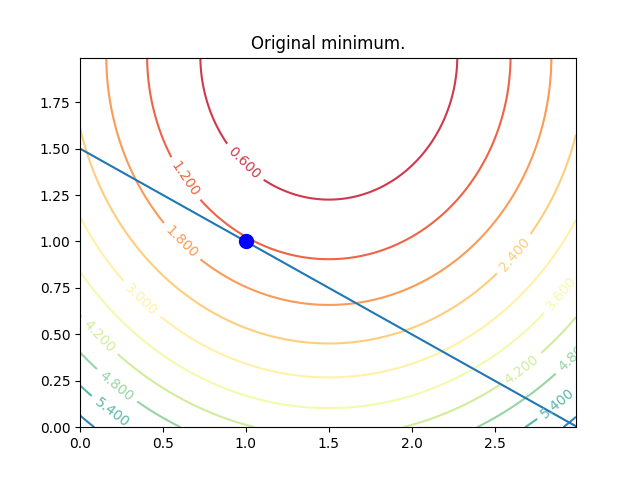
\includegraphics[width=\textwidth]{../img/original-minimum.png}
    \caption{Original minimum.}
    \label{fig:first}
  \end{subfigure}
  \hfill
  \begin{subfigure}{0.45\textwidth}
    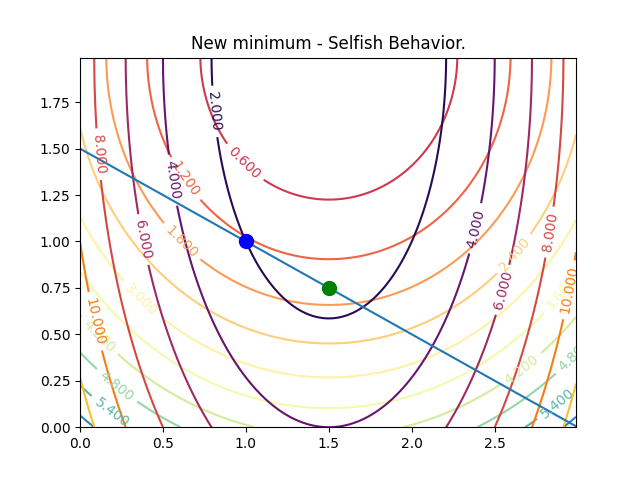
\includegraphics[width=\textwidth]{../img/new-minimum-selfish.png}
    \caption{Minimum after non-conforming behavior.}
    \label{fig:second}
  \end{subfigure}
  \caption{Effects of non-conforming behaviors on optimal value. \todo{Refaire les images}}
  \label{fig:figures}
\end{figure}



\printbibliography

\chapter{Towards Safe algorithms}

\epigraph{\centering Trust is an illusion, \\M'Lady. \\I believe only in \\mutual self-interest.}
{\textit{Jupiter Ascending}\\\textsc{The Wachowskis}}

\minitoc
General discussion about ways to secure negotiation, here we discuss what
\begin{description}
  \item[Discussion about Methods]
  \item[Discussion about Detection and Isolation]
        \begin{description}
          \item[Learning methods] Use input labeled data to train detector
          \item[Analytical methods] Use model of the system and residuals
        \end{description}
  \item[Discussion about Recovery] Could show different cases
        \begin{description}
          \item[Active methods] Need detection
          \item[Passive methods] Robust control
        \end{description}


\end{description}


\begin{figure}[h]
  \centering
  \begin{subfigure}{0.45\textwidth}
    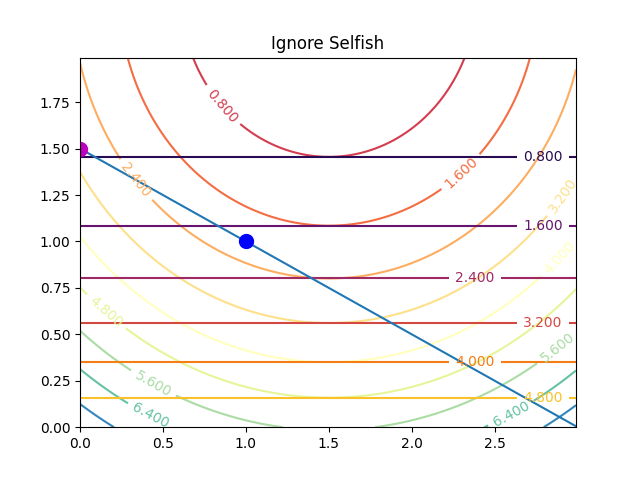
\includegraphics[width=\textwidth]{../img/ignoreX.png}
    \caption{Optimal value after ignoring attacker.}
    \label{fig:third}
  \end{subfigure}
  \hfill
  \begin{subfigure}{0.45\textwidth}
    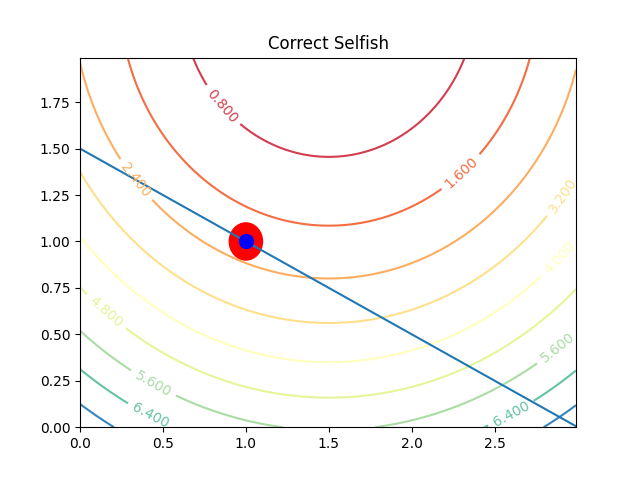
\includegraphics[width=\textwidth]{../img/correctX.png}
    \caption{Optimal value after trying to recover original behavior.}
    \label{fig:third}
  \end{subfigure}

  \caption{Recovering options.}
  \label{fig:figures}
\end{figure}


Model 3R-2C \cite{GoudaEtAl2002}
\begin{figure}[h]
  \centering
  \begin{circuitikz}[european]
    \draw (0,0) node[tlground]{} to[isource, l=$P^{\text{heat}}$] ++(0,2)
    to[short, -*] ++(1.5,0) coordinate (a);

    \draw (a) node[above]{$T^{\text{in}}$}  to[C=$C^{\text{air}}$] ++(0,-2) node[tlground]{};
    \draw (0,-3) node[tlground]{} to[isource, l=$I^{\text{sol}}$] ++(0,2)
    to[short, -*] ++(1.5,0) coordinate (b);
    \draw (b) to[C=$C^{\text{walls}}$] ++(0,-2) node[tlground]{};

    \draw (a) -- ++(2,0) coordinate (c) -- ++(0,-.5) to[R=$R^{\text{iw/ia}}$] ++(0,-2) -- ++(0,-.5) coordinate (d);

    \draw (b) node[above]{$T^{\text{walls}}$} to[short,-*] (d);

    \draw (c) --  ++(2.5,0) -- ++(0,-.5) to[R=$R^{\text{oa/ia}}$] ++(0,-2) -- ++(0,-.5) coordinate (e);

    \draw (d) to[R=$R^{\text{ow/oa}}$] (e) to[battery,l=$T^{\text{out}}$] ++(0,-2) node[tlground]{};
  \end{circuitikz}
  \caption{Thermic Model 3R-2C of a room.}
  \label{fig:3R2C_model}
\end{figure}

The state-space model of each subsystem is given by:
\begin{equation}
  \begin{matrix}
    \label{eq:systems_cont}
    \dot{\vec{x}}_{i}(t)  &=&{A_{c}}_{i}\vec{x}_{i}(t) &+& {B_{c}}_{i}\vec{u}_{i}(t)\\
    \vec{y}_{i}(t)        &=&{C_{c}}_{i}\vec{x}_{i}(t) &&
  \end{matrix},
\end{equation}
where
\begin{equation}
  \label{eq:4}
  \begin{matrix}
    A_{\mathrm{c}_{i}}=\left[
      \begin{matrix}
        -\frac{1}{C^{\text{walls}}_{i}R^{\text{oa/ia}}_{i}}-\frac{1}{C^{\text{walls}}_{i}R^{\text{iw/ia}}_{i}}& \frac{1}{C^{\text{walls}}_{i}R^{\text{iw/ia}}_{i}}\\
        \frac{1}{C^{\text{air}}_{i}R^{\text{iw/ia}}_{i}} &-\frac{1}{C^{\text{air}}_{i}R^{\text{ow/oa}}o_{i}}-\frac{1}{C^{\text{air}}_{i}R^{\text{iw/ia}}_{i}}
      \end{matrix}\right]\\
    \begin{matrix}
      B_{\mathrm{c}_{i}}=\left[
        \begin{matrix}  \frac{10}{C^{\text{walls}}_{i}}& 0\end{matrix}
      \right]\T&C_{\mathrm{c}_{i}}=\left[\begin{matrix}1 & 0\end{matrix}\right]
    \end{matrix}
  \end{matrix}
\end{equation}
where ${\vec{x}_{i}=[{{x}_{A}}_{i}\T\ {{x}_{W}}_{i}\T]\T}$. ${x_A}_i$ and ${x_W}_i$ are the mean temperatures of the air and walls inside room~$i$. $\vec{u}_{i}$ is the input (the heating power)
for the corresponding room. The inputs are constraint by ${\sum_{i=1}^{4}\vec{u}_{i}(t)\preceq 4\mathrm{kW}}$.

\begin{table}[b]
  \centering
  \caption{Model Parameters}\label{tab:modelParamMeaning}
  \begin{tabular}[b]{cl}
    \toprule
    Symbol&Meaning\\
    \midrule
    $C^{\text{air}}_{i}$  &Heat Capacity of Inside Air\\
    $C^{\text{walls}}_{i}$ &Heat Capacity of External Walls\\
    $R^{\text{iw/ia}}_{i}$ &Resist. Between Inside Air and Inside Walls\\
    $R^{\text{ow/oa}}_{i}$ &Resist. Between Outside Air and Outside Walls\\
    $R^{\text{oa/ia}}_{i}$ &Resist. Between Inside and Out.\ Air (from windows)\\
    \bottomrule
  \end{tabular}
\end{table}

\begin{table}[b]
  \centering
  \caption{
    Parameters for each agent}\label{tab:modelParam}
  \begin{tabular}[t]{cccccc} \toprule
    Symbol& I & II & III & IV &Unit\\
    \midrule
    $C^{\text{walls}}$   &$5.4$&$4.9$&$4.7$&$4.7$ &$10^{4}\mathrm{J/K}$ \\
    $C^{\text{air}}$     &$7.5$ &$8.4 $&$8.2$ &$7.7$&$10^{4}\mathrm{J/K}$  \\
    $R^{\text{oa/ia}}$   &$5.2$&$4.6$&$4.9$&$5.4$&$10^{-3}\mathrm{K/W}$ \\
    $R^{\text{iw/ia}}$   &$2.3$&$2.4$&$2.3$&$2.9$&$10^{-4}\mathrm{K/W}$\\
    $R^{\text{ow/oa}}$   &$1.5$&$0.6$&$0.7$&$0.7$& $10^{-4}\mathrm{K/W}$ \\
    \bottomrule
  \end{tabular}
\end{table}
\todo{References }

\end{document}
